\begin{frame}{Dangle and cut edges}
    \begin{itemize}
        \item We extend the overlay DCEL approach to accept scattered and noisy line segments (including dangles and cut edges) as input, rather than being restricted to clean polygon data.
        \item This chapter extends the previous work in [Calderon et al, 2023]\footnote{Scalable Overlay Operations over DCEL Polygon Layers.(SSTD'23).} by building on the scalable polygonization methods presented in [Abdelhafeez et al, 2023]\footnote{DDCEL: Efficient Distributed Doubly Connected Edge List for Large Spatial Networks. (MDM'23).}.
    \end{itemize}
\end{frame}

\begin{frame}{Dangle and cut edges}
    \centering
    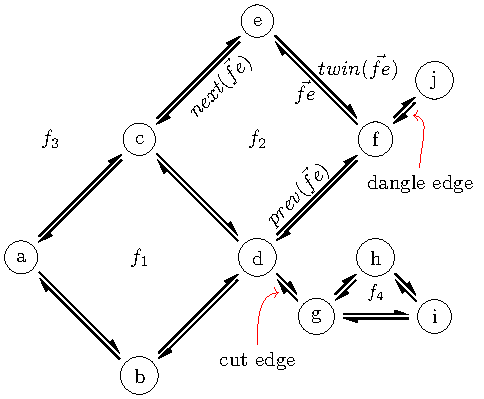
\includegraphics[width=0.6\textwidth]{../thesis/chapterExtension/dcel_example2}
\end{frame}

\begin{frame}{Implementation}
    \begin{itemize}
        \item The \textbf{DDCEL Construction} consists of two primary phases:
            \begin{itemize}
                \item Generation Phase \textbf{(Gen Phase)} 
                \item Remaining Phase (Rem Phase)
            \end{itemize}
        \item Optimization Step: Replace the Rem Phase with the optimization of faces spanning multiple cells based on \textit{Face ID}.
    \end{itemize}
\end{frame}

\begin{frame}{Gen Phase}
    \centering

    \begin{tikzpicture}
    \node (A) {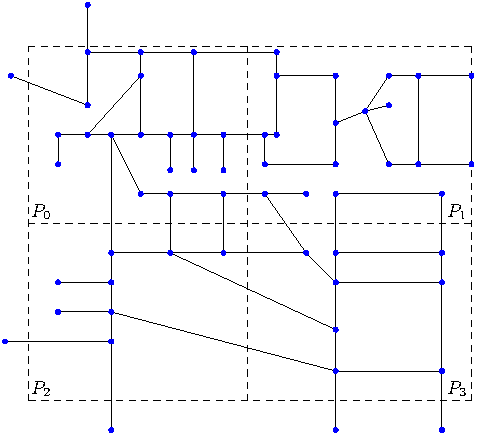
\includegraphics[width=0.8\textheight]{../thesis/chapterExtension/model/input/input}};
    \pause
    \draw[white, fill=white] (-4,-4) rectangle (4,4);
    \node (B) {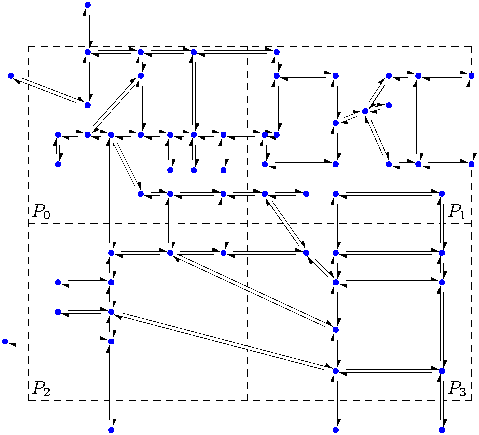
\includegraphics[width=0.8\textheight]{../thesis/chapterExtension/model/a/a}};
    \pause
    \draw[white, fill=white] (-4,-4) rectangle (4,4);
    \node (C) {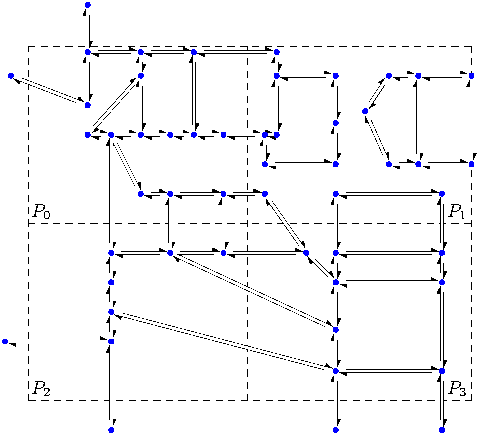
\includegraphics[width=0.8\textheight]{../thesis/chapterExtension/model/b/b}};
    \pause
    \draw[white, fill=white] (-4,-4) rectangle (4,4);
    \node (D) {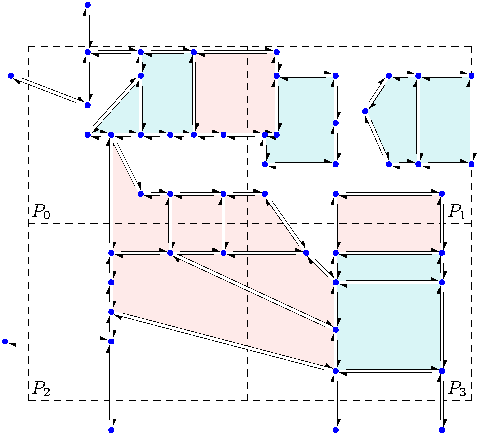
\includegraphics[width=0.8\textheight]{../thesis/chapterExtension/model/c/c}};
    \end{tikzpicture}
\end{frame}

\begin{frame}{Reduce by ID re-partition}
    \centering
    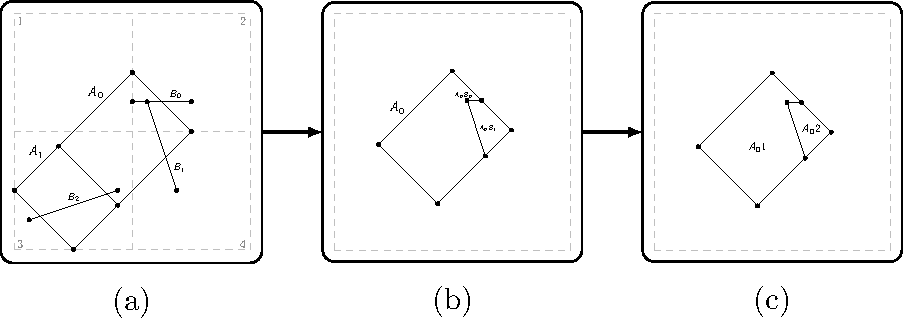
\includegraphics[width=\textwidth]{../thesis/chapterExtension/dangles_cuts/DAC}
\end{frame}

\begin{frame}{Dangle and cut edges}
    \centering
    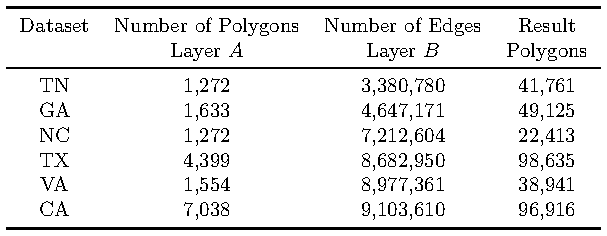
\includegraphics[width=0.85\textwidth]{figures/dangles_datasets}
\end{frame}

\begin{frame}{Dangle and cut edges}
    \centering
    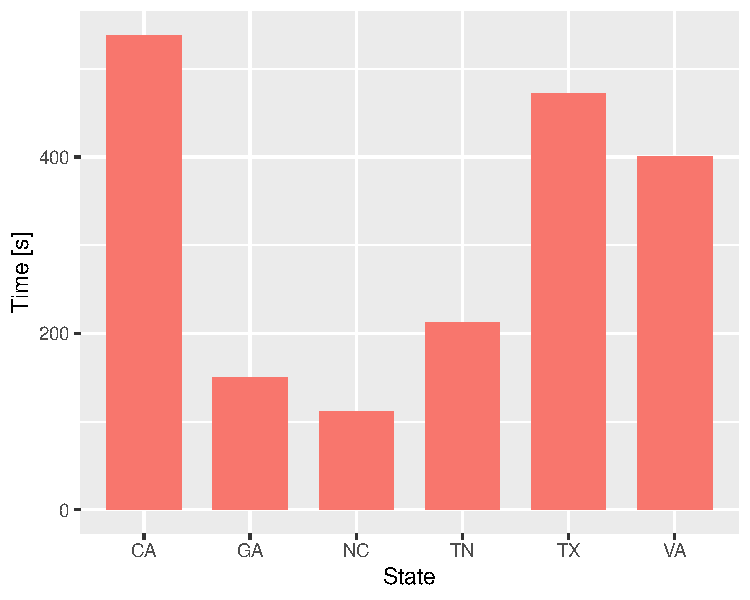
\includegraphics[width=0.75\textwidth]{../thesis/chapterExtension/states}
\end{frame}
